\documentclass{article}
\usepackage{fleqn}
\usepackage{epsf}
\usepackage{aima2e-slides}
\usepackage{graphicx}
\usepackage{listings}

\usepackage[landscape]{geometry}

%\usepackage{amsmath}
\usepackage{amssymb}

\newcommand{\mm}{\!\!-\!\!}
\newcommand{\prompt}{$> \ $}
\newcommand{\rep}[1]{\ulcorner #1 \urcorner}

\begin{document}

\begin{huge}
\titleslide{Chapter 8. Modules \\ (Essentials of Programming Languages)}{Kwanghoon Choi \\ \ \\ Software Languages and Systems Laboratory\\ Chonnam National University}

\sf

%%%%%%%%%%%% Slide %%%%%%%%%%%%%%%%%%%%%%%%%%%%%%%%%%%%%%%%%%%%%%%%%%%
\heading{Outline}

This chapter discusses modules that we will need when we are to build larger systems with thousands of lines of code.

\blob The Simple Module System

\blob Modules That Declare Types

\blob Module Procedures

%%%%%%%%%%%% Slide %%%%%%%%%%%%%%%%%%%%%%%%%%%%%%%%%%%%%%%%%%%%%%%%%%%
\heading{Introduction}

When we are to build large systems, it is desirable to have:

\begin{itemize}
\item A way to separate the system into self-contained parts, and to document the dependencies between those parts
\item A way to control the scope and binding of names 
\item A way to enforce abstraction boundaries 
\item A way to combine these parts flexibly so that a single part may be reused in different contexts.
\end{itemize}

$\Rightarrow$ Modules \& type systems for modules (to create and enforce abstraction boundaries)

%%%%%%%%%%%% Slide %%%%%%%%%%%%%%%%%%%%%%%%%%%%%%%%%%%%%%%%%%%%%%%%%%%
\heading{Introduction (Cont.)}

A program = a sequence of module definitions + a main expression

\begin{itemize}
\item Each definition binds a name to a module
\item A created module is either 
\begin{itemize}
\item a simple module (a set of bindings like an environment) or
\item a module procedure (taking a module and producing another)
\end{itemize}
\item Each module has an interface as:
\begin{itemize}
\item a simple interface (listing the module bindings and their types)
\item a module procedure interface (specifying 
\begin{itemize}
\item the interface of the argument module interface and 
\item the interface of the result module)
\end{itemize}
\end{itemize}
\end{itemize}

Module interfaces determine the ways in which modules can be combined.


%%%%%%%%%%%% Slide %%%%%%%%%%%%%%%%%%%%%%%%%%%%%%%%%%%%%%%%%%%%%%%%%%%
\heading{8.1 The Simple Module System}
Alice's view of the three modules in the project
\begin{center}
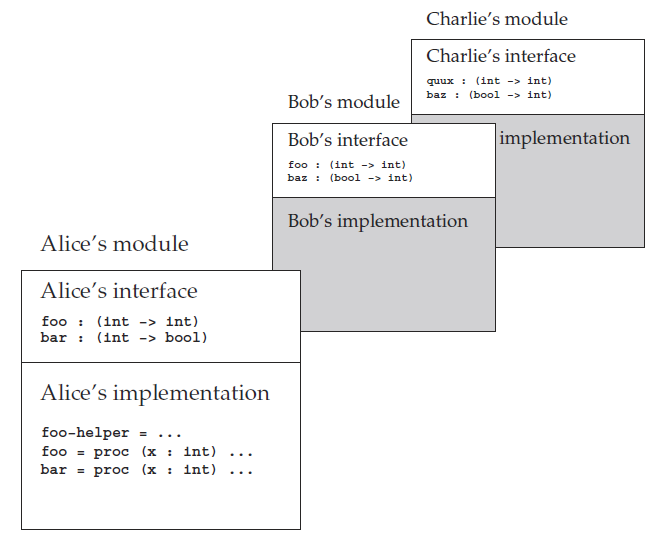
\includegraphics[width=0.7\linewidth]{eopl3_figure8_1}
\end{center}

%%%%%%%%%%%% Slide %%%%%%%%%%%%%%%%%%%%%%%%%%%%%%%%%%%%%%%%%%%%%%%%%%%
\heading{8.1.1 Examples}

SIMPLE-MODULES: a language with only simple modules (and no module procedures)

\begin{lstlisting}[language=Lisp]
module m1 
  interface [a:int b:int c:int]
  body [  a = 33
          x = -(a,1) 
          b = -(a,x)
          c = -(x,b) ]
  let a = 10
  in -(-(from m1 take a, 
          from m1 take b),      a)    
\end{lstlisting}

%%%%%%%%%%%% Slide %%%%%%%%%%%%%%%%%%%%%%%%%%%%%%%%%%%%%%%%%%%%%%%%%%%
\heading{8.1.1 Examples}

Some of the scopes for a simple module
\begin{center}
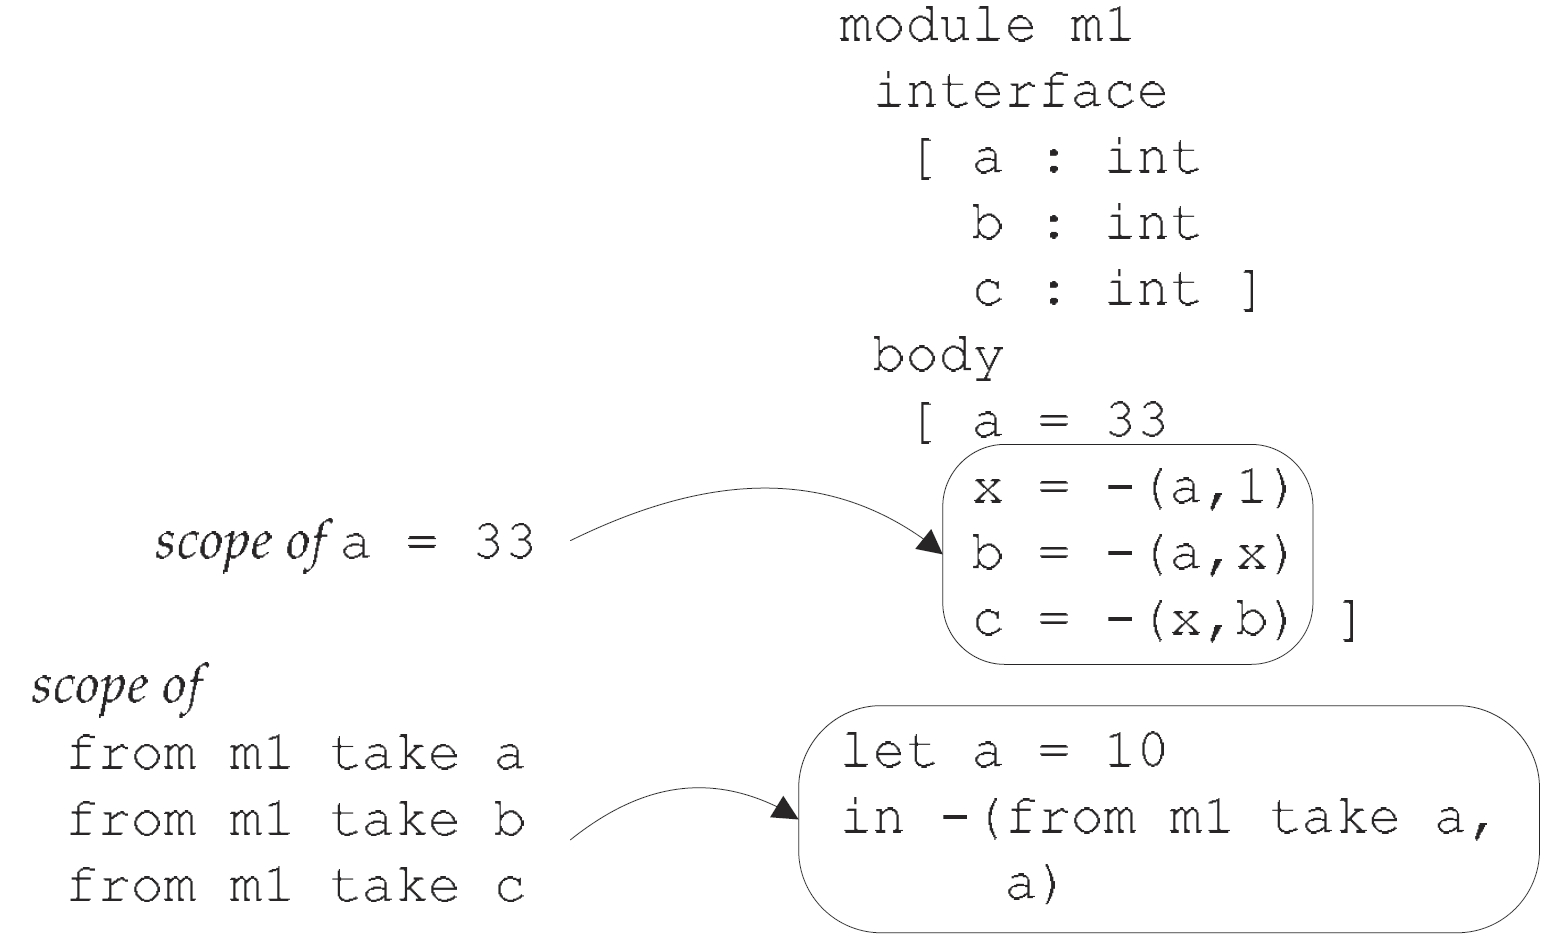
\includegraphics[width=0.85\linewidth]{eopl3_figure8_2}
\end{center}

cf. let$^*$ scoping (Exercise 3.17)

%%%%%%%%%%%% Slide %%%%%%%%%%%%%%%%%%%%%%%%%%%%%%%%%%%%%%%%%%%%%%%%%%%
\heading{8.1.1 Examples (Cont.)}

In the previous example,
\begin{itemize}
\item The body {\it implements} the interface.
\begin{itemize}
\item The interface {\it offers} (or {\it advertises} or {\it promises}) three integer values.
\item The body {\it supplies} (or {\it provoides} or {\it exports}) these values.
\item A module body {\it satisfies} an interface when it supplies a value of the advertised type for each of the variables that are named in the interface.
\end{itemize}
\end{itemize}

%%%%%%%%%%%% Slide %%%%%%%%%%%%%%%%%%%%%%%%%%%%%%%%%%%%%%%%%%%%%%%%%%%
\heading{8.1.1 Examples (Cont.)}

In the previous example (Cont.),
\begin{itemize}
\item The scoping technology does not scale to the module program.
\begin{itemize}
\item {\it Qualified variables} vs. simple variables
\begin{itemize}
\item `from m1 take x' vs. x
\end{itemize}
\end{itemize}
\item Each module establishes an abstraction boundary between the module body
and the rest of the program. 
\begin{itemize}
\item The expressions in the module body are {\it inside} the abstraction boundary
\item Everything else is {\it outside} the abstraction boundary.
\begin{itemize}
\item `from m1 take x' is not in scope
\end{itemize}
\end{itemize}
\end{itemize}

%%%%%%%%%%%% Slide %%%%%%%%%%%%%%%%%%%%%%%%%%%%%%%%%%%%%%%%%%%%%%%%%%%
\heading{8.1.1 Examples (Cont.)}

\begin{minipage}[t]{.5\textwidth}
An ill-typed module
\begin{itemize}
\item
\begin{lstlisting}[language=Lisp]
module m1 
  interface [u:bool]
  body [u=33]
\end{lstlisting}
\end{itemize}

On ordering of bindings
\begin{itemize}
\item
\begin{lstlisting}[language=Lisp]
module m1 
  interface [
    u:int v:int]
  body [v=33 u=44]
\end{lstlisting}
\end{itemize}
\end{minipage}
\begin{minipage}[t]{.5\textwidth}
Two modules in a correct order
\begin{itemize}
\item
\begin{lstlisting}[language=Lisp]
module m1 
  interface [u:int]
  body [u=44]
  
module m2
  interface [v:int]
  body [
    v=-(from m1 take u, 11)]
  
-(from m1 take u, 
  from m2 take v)  
\end{lstlisting}
\end{itemize}
\end{minipage}

%%%%%%%%%%%% Slide %%%%%%%%%%%%%%%%%%%%%%%%%%%%%%%%%%%%%%%%%%%%%%%%%%%
\heading{8.1.1 Examples (Cont.)}

\begin{minipage}[t]{.5\textwidth}
The two modules in an incorrect order
\begin{itemize}
\item
\begin{lstlisting}[language=Lisp]
module m2
  interface [v:int]
  body [
    v=-(from m1 take u, 11)]
    
module m1 
  interface [u:int]
  body [u=44]
    
-(from m1 take u, 
  from m2 take v)  
\end{lstlisting}
\end{itemize}
\end{minipage}

%%%%%%%%%%%% Slide %%%%%%%%%%%%%%%%%%%%%%%%%%%%%%%%%%%%%%%%%%%%%%%%%%%
\heading{8.1.2 Implementing the Simple Module System}

Syntax - module and interface
\begin{itemize}
\item Program ::= \{ModuleDefn\}$^*$ Expression \\
   \fbox{a-program (m-defs body)} \\
\item ModuleDefn ::= module Identifier interface Iface body ModuleBody \\
	\fbox{a-module-definition (m-name expected-iface m-body)}
\item Iface ::= [ \{Decl\}$^*$ ] \\
	\fbox{simple-iface (decls)}
\item Decl ::= Identifier : Type \\
	\fbox{val-decl (var-name ty)}
\end{itemize}

%%%%%%%%%%%% Slide %%%%%%%%%%%%%%%%%%%%%%%%%%%%%%%%%%%%%%%%%%%%%%%%%%%
\heading{8.1.2 Implementing the Simple Module System (Cont.)}

Syntax - module body
\begin{itemize}
\item ModuleBody ::= [ \{Defn\}$^*$ ] \\
	\fbox{val-defn (var-name exp)}
\item Defn ::= Identifier = Expression \\
	\fbox{val-defn (var-name exp)}
\item Expression ::= from Identifier take Identifier \\
	\fbox{qualified-var-exp (m-name var-name)}
\end{itemize}

%%%%%%%%%%%% Slide %%%%%%%%%%%%%%%%%%%%%%%%%%%%%%%%%%%%%%%%%%%%%%%%%%%
\heading{8.1.2 Implementing the Simple Module System (Cont.)}

The Interpreter
\begin{itemize}
\item Evaluation of a module body will produce a {\it module}, which is
an environment consisting of all the bindings exported by the module.
\end{itemize}

\begin{lstlisting}[language=Lisp]
(define-datatype typed-module typed-module?
  (simple-module
    (bindings environment?)))  
    
(define-datatype environment environment?
  .... as before ...
  (extended-env-with-module 
    (m-name symbol?)
    (m-val typed-module?)
    (saved-env environment?)))
\end{lstlisting}

%%%%%%%%%%%% Slide %%%%%%%%%%%%%%%%%%%%%%%%%%%%%%%%%%%%%%%%%%%%%%%%%%%
\heading{8.1.2 Implementing the Simple Module System (Cont.)}

\begin{minipage}[t]{.43\textwidth}
\begin{lstlisting}[language=Lisp]
module m1
 interface
  [a:int b:int c:int]
 body[a=33 b=44 c=55]

module m2
 interface
  [a:int b:int]
 body [a=66 b=77]

let z=99 in
 -(z, 
  -(from m1 take a,
    from m2 take a))
\end{lstlisting}          
\end{minipage}
\begin{minipage}[t]{.5\textwidth}
\begin{lstlisting}[language=Lisp]
(extended-env z (num-val 99)
 (exnteded-env-with-module
  m2 
  (extended-env a (num-val 66)
   (extended-env b (num-val 77)
    (empty-env)))
  (empty-env))
  (extended-env-with-module
   m1
   (extended-env a (num-val 33)
    (extended-env b (num-val 44)
     (extended-env c (num-val 55))))
   (empty-env))
  (empty-env))
\end{lstlisting}   
\end{minipage}

%%%%%%%%%%%% Slide %%%%%%%%%%%%%%%%%%%%%%%%%%%%%%%%%%%%%%%%%%%%%%%%%%%
\heading{8.1.2 Implementing the Simple Module System (Cont.)}

Procedures for the interpreter in Figure 8.3 and 8.4
\begin{itemize}
\item lookup-qualified-var-in-env : looking up the module 
in the current environment and then the variable in the module environment
\item value-of-program : adding module definitions to the environment
\begin{itemize}
\item add-module-defns-to-env
\end{itemize}
\item value-of-module-body : producing an environment containing only the bindings
produced by the definitions
\begin{itemize}
\item defns-to-env
\end{itemize}
\end{itemize}

%%%%%%%%%%%% Slide %%%%%%%%%%%%%%%%%%%%%%%%%%%%%%%%%%%%%%%%%%%%%%%%%%%
\heading{8.1.2 Implementing the Simple Module System (Cont.)}

The Checker
\begin{itemize}
\item Making sure that each module body satisfies its interface, and that each
variable is used consistently with its type.
\item Our language follows let$^*$ scoping putting into scope qualified variables for each of the bindings exported by the module.
\end{itemize}


%%%%%%%%%%%% Slide %%%%%%%%%%%%%%%%%%%%%%%%%%%%%%%%%%%%%%%%%%%%%%%%%%%
\heading{8.1.2 Implementing the Simple Module System (Cont.)}

In type environment, each module name is bound to its interface.

\begin{lstlisting}[language=Lisp]
(define-datatype type-environment type-environment?
  .... as before ...
  (extended-tenv-with-module 
    (name symbol?)
    (interface interface?)
    (saved-tenv type-environment?)))
\end{lstlisting}

%%%%%%%%%%%% Slide %%%%%%%%%%%%%%%%%%%%%%%%%%%%%%%%%%%%%%%%%%%%%%%%%%%
\heading{8.1.2 Implementing the Simple Module System (Cont.)}

Procedures for the interpreter in Figure 8.5, 8.6, and 8.7.
\begin{itemize}
\item looku-qualified-var-in-tenv : looking up the type of the module name and then the type of the variable
\item type-of-program : adding module interfaces to the type environment
\begin{itemize}
\item add-module-defns-to-tenv
\end{itemize}
\item \textless:-iface : checking if the interface produced by the module body matches the advertised interface
\begin{itemize}
\item \textless:-decls
\end{itemize}
\end{itemize}


%%%%%%%%%%%% Slide %%%%%%%%%%%%%%%%%%%%%%%%%%%%%%%%%%%%%%%%%%%%%%%%%%%
\heading{8.1.2 Implementing the Simple Module System (Cont.)}

An interface produced by the module body

\begin{minipage}[t]{.5\textwidth}
\begin{lstlisting}[language=Lisp]
[ a = 33
  x = -(a,1)
  b = -(a,x)
  c = -(x,b) ]
\end{lstlisting}   
\end{minipage}
\begin{minipage}[t]{.5\textwidth}
\begin{lstlisting}[language=Lisp]
[ a : int
  x : int
  b : int
  c : int ]
\end{lstlisting}   
\end{minipage}

The produced interface matches the advertise interface

\begin{minipage}[t]{.25\textwidth}
\begin{lstlisting}[language=Lisp]
[ a : int   
  x : int   
  b : int   
  c : int ]
\end{lstlisting}   
\end{minipage}
\begin{minipage}[t]{.5\textwidth}
\begin{lstlisting}[language=Lisp]
<:    [ a:int 
        b:int 
        c:int] 
\end{lstlisting}   
\end{minipage}

%%%%%%%%%%%% Slide %%%%%%%%%%%%%%%%%%%%%%%%%%%%%%%%%%%%%%%%%%%%%%%%%%%
\heading{8.1.2 Implementing the Simple Module System (Cont.)}

The procedure \textless:-decls in Figure 8.7
\begin{itemize}
\item If decls1 and decls2 are two sets of declarations, 
\begin{itemize}
\item decls1 \textless:- decls2 if and only if any module that supplies bindings for the declarations in decls1 also supplies bindings for the declarations in decls2.
\end{itemize}
\end{itemize}


%%%%%%%%%%%% Slide %%%%%%%%%%%%%%%%%%%%%%%%%%%%%%%%%%%%%%%%%%%%%%%%%%%
\heading{8.2 Modules That Declare Types}

So far, our interfaces have declared only ordinary variables and their types. In the next module language, OPAQUE-TYPES, we allow interfaces to declare types as well.

%%%%%%%%%%%% Slide %%%%%%%%%%%%%%%%%%%%%%%%%%%%%%%%%%%%%%%%%%%%%%%%%%%
\heading{8.2.1 Examples} 

Alice provides interfaces for pairs of integers, representing the x- and y- coordinates of a point.

\begin{lstlisting}[language=Lisp]
module Alices-points
 interafce
  [transparent point = pairof int * int
   initial-point : (int -> point)
   increment-x : (point -> point)
   get-x : (point -> int)
   ... ]
\end{lstlisting}   

Using a module of this interface,
\begin{lstlisting}[language=Lisp]
[transparent point = from Alices-points take point
  foo = proc (p1 : point)
         proc (p2 : point) ...
  ... ]
\end{lstlisting}   

%%%%%%%%%%%% Slide %%%%%%%%%%%%%%%%%%%%%%%%%%%%%%%%%%%%%%%%%%%%%%%%%%%
\heading{8.2.1 Examples (Cont.)} 

Bob can write a procedure depending on the implementation of pairs while Alice decides to change the representation of points so that the the y-coordinate is in the first component.

\begin{lstlisting}[language=Lisp]
     increment-y = proc (p : point)
                 unpair x y = p
                 in newpair(x, -(y, -1))
\end{lstlisting}   

Alice can solve her problem by making point an {\it opaque} data type.

\begin{lstlisting}[language=Lisp]
     opaque point
       initial-point : (int -> point)
       increment-x : (point -> point)
       get-x : (point -> int)
\end{lstlisting}   

Then Bob can no longer manipulate points using any procedures other than the ones in Alice's interface.

%%%%%%%%%%%% Slide %%%%%%%%%%%%%%%%%%%%%%%%%%%%%%%%%%%%%%%%%%%%%%%%%%%
\heading{8.2.1 Examples: Transparent Types} 

Transparent type declarations (also called concrete type declarations or {\it type abbreviations})

\begin{lstlisting}[language=Lisp]
module m1
  interface
   [ transparent t = int
     z : t
     s : (t -> t)
     is-z? : (t -> bool) ]
  body
   [ type t = int
     z = 33
     s = proc (x : t) -(x, -1)
     is-z? = proc (x : t) zero? ( -(x,z)) ]
  proc (x : from m1 take t)
    (from m1 take is-z? -(x, 0))
\end{lstlisting}   


%%%%%%%%%%%% Slide %%%%%%%%%%%%%%%%%%%%%%%%%%%%%%%%%%%%%%%%%%%%%%%%%%%
\heading{8.2.1 Examples: Opaque Types} 

Opaque type declarations (sometimes called {\it abstract} types)

\begin{lstlisting}[language=Lisp]
module m1
  interface
   [ opaque t
     z : t    s : (t -> t)    is-z? : (t -> bool) ]
  body
   [ type t = int
     z = 33
     s = proc (x : t) -(x, -1)
     is-z? = proc (x : t) zero? ( -(x,z)) ]
  proc (x : from m1 take t)
    (from m1 take is-z? -(x, 0))
\end{lstlisting}   

-(x,0) is ill-typed!

%%%%%%%%%%%% Slide %%%%%%%%%%%%%%%%%%%%%%%%%%%%%%%%%%%%%%%%%%%%%%%%%%%
\heading{8.2.1 Examples: Opaque Types (Cont.)} 

This is the abstraction boundary. The definition of the opaque type t is hidden from the rest of 
the program.

\begin{lstlisting}[language=Lisp]
module m1
  interface
   [ opaque t
     z : t    s : (t -> t)    is-z? : (t -> bool) ]
  body
   [ type t = int
     z = 33
     s = proc (x : t) -(x, -1)
     is-z? = proc (x : t) zero? ( -(x,z)) ]
  proc (x : from m1 take t)
    (from m1 take is-z? x)
\end{lstlisting}  

Example 8.8 ~ 8.13


%%%%%%%%%%%% Slide %%%%%%%%%%%%%%%%%%%%%%%%%%%%%%%%%%%%%%%%%%%%%%%%%%%
\heading{8.2.2 Implementation: Syntax}

Transparent and opaque type decls and qualified type references

Syntax 
\begin{itemize}
\item Type ::= Identifier \\
	\fbox{named-type (name)}
\item Type ::= from Identifier take Identifier \\
	\fbox{qualified-type (m-name t-name)}
\item Decl ::= opaque Identifier \\
	\fbox{opaque-type-decl (t-name)}
\item Decl ::= transparent Identifier = Type \\
	\fbox{transparent-type-decl (t-name ty)}	
\item Defn ::= type Identifier = Type \\
	\fbox{type-defn (name ty)}
\end{itemize}



%%%%%%%%%%%% Slide %%%%%%%%%%%%%%%%%%%%%%%%%%%%%%%%%%%%%%%%%%%%%%%%%%%
\heading{8.2.2 Implementation: Interpreter}

Interpreter

\begin{itemize}
\item The interpreter doesn't look at types or declarations, so the only change to the interpreter is to make it
ignore type definitions.
\begin{itemize}
\item defns-to-env 
\end{itemize}
\end{itemize}


%%%%%%%%%%%% Slide %%%%%%%%%%%%%%%%%%%%%%%%%%%%%%%%%%%%%%%%%%%%%%%%%%%
\heading{8.2.2 Implementation: The Checker}

The Checker

To handle opaque and transparent types in a systematic way, we use expanded type as
\begin{itemize}
\item Type ::= int $|$ bool $|$ from m take t $|$ Type $\rightarrow$ Type
\end{itemize}

Our type environments will bind each named type or qualified type to an expanded type. 

\begin{lstlisting}[language=Lisp]
(define-datatype type-environment type-environment?
  ... as before ...
  (extend-tenv-with-type
    (name type?)
    (type type?)
    (saved-tenv type-environment?)))
\end{lstlisting}  


%%%%%%%%%%%% Slide %%%%%%%%%%%%%%%%%%%%%%%%%%%%%%%%%%%%%%%%%%%%%%%%%%%
\heading{8.2.2 Implementation: The Checker (Cont.)}

A procedure, expand-type (ty, tenv) = expanded-type

\begin{itemize}
\item
In type-of in the checker, we always use (extend-tenv var (expanded-type ty tenv) tenv)
\item
When we process a list of definitions with defns-to-decls, we expand its right-hand side and add it to the type environment.
\item
Where we add a module to the type environment, in add-module-defns-to-tenv, we need to expand the interface to the type environment (Figure 8.9)
\begin{itemize}
\item expand-iface (Figure 8.9)
\item This calls expand-decls  (Figure 8.10)
\end{itemize}
\end{itemize}

%%%%%%%%%%%% Slide %%%%%%%%%%%%%%%%%%%%%%%%%%%%%%%%%%%%%%%%%%%%%%%%%%%
\heading{8.2.2 Implementation: The Checker (Cont.)}

Lastly, we modify  \textless:-decls to handle the two new kinds of declarations as (Figure 8.11): 
\begin{itemize}
\item They are both value declarations, and their types match.
\item They are both opaque type declarations.
\item They are both transparent type declarations, and their defs match.
\item decl1 is a transparent type declaration, and decl2 is an opaque type declaration.
\begin{itemize}
\item (transparent t = int) \textless: (opaque t)
\item (opaque t) $\not$\textless:  (transparent t = int) 
\end{itemize}
\end{itemize}

equiv-type? compares two types in their expanded form. (Figure 8.12)

%%%%%%%%%%%% Slide %%%%%%%%%%%%%%%%%%%%%%%%%%%%%%%%%%%%%%%%%%%%%%%%%%%
\heading{8.3 Module Procedures}

In OPAQUE-TYPES, the programs have a fixed set of dependencies, 
which are sometimes hard-coded. 

Hard-coded dependencies lead to bad program design because they make it
difficult to reuse modules.

A solution is module procedures.



%%%%%%%%%%%% Slide %%%%%%%%%%%%%%%%%%%%%%%%%%%%%%%%%%%%%%%%%%%%%%%%%%%
\heading{8.3.1 Examples}

Charlie wants to use Alice's module with Diana's database module.
How could you rewrite Alice's module in a modular way?

\begin{center}
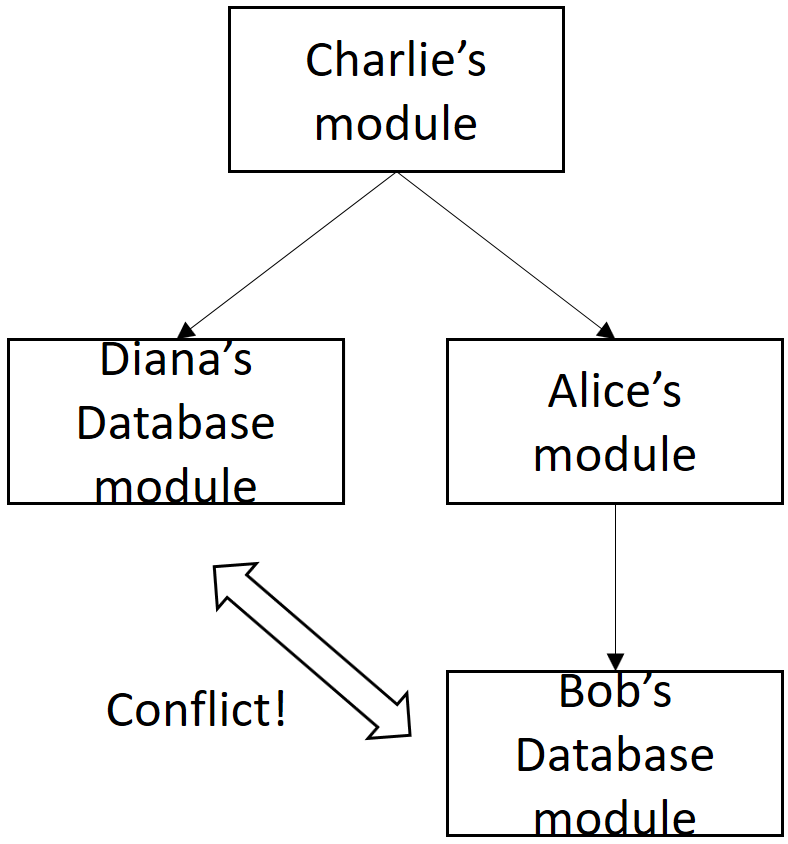
\includegraphics[width=0.5\linewidth]{eopl3_ch8_module_conflicts}
\end{center}


%%%%%%%%%%%% Slide %%%%%%%%%%%%%%%%%%%%%%%%%%%%%%%%%%%%%%%%%%%%%%%%%%%
\heading{8.3.1 Examples (Cont.)}

To make this possible in a modular way, Alice rewrites her code using
{\it module procedures} (sometimes called parameterized modules). 

A module procedure is like a procedure, except that it works with modules,
rather than with expressed values.
\begin{itemize}
\item modules vs. expressed values
\item interfaces (of modules) vs. types (of expressed values)
\end{itemize}

Q. Explain how a module procedure solves the conflict in the previous
example.

PROC-MODULES, a language with module procedures

%%%%%%%%%%%% Slide %%%%%%%%%%%%%%%%%%%%%%%%%%%%%%%%%%%%%%%%%%%%%%%%%%%
\heading{8.3.1 Examples (Cont.)}

A module procedure, Alices-point-builder begins with
\begin{lstlisting}[language=Lisp]
module Alices-point-builder
 interface
  ( (database : [opaque db-type
     opaque node-type
     insert-node : (node-type -> (db-type -> db-type)) ])
     => [opaque point
         initial-point : (int -> point) ] )
 body  ...      
\end{lstlisting} 

\begin{itemize}
\item In Alices-points, (Alices-point-builder Bobs-db-module)
\item In Charlies-points, (Alices-point-builder Dianas-db-module)
\end{itemize}

%%%%%%%%%%%% Slide %%%%%%%%%%%%%%%%%%%%%%%%%%%%%%%%%%%%%%%%%%%%%%%%%%%
\heading{8.3.1 Examples (Cont.)}

\begin{lstlisting}[language=Lisp]
module Alices-point-builder
 interface
  ((database : [opaque db-type
     opaque node-type
     insert-node : (node-type -> (db-type -> db-type)) ])
  => [opaque point
      initial-point : (int -> point) ])
 body
  module-proc (m : [opaque db-type
     opaque node-type
     insert-node : (node-type -> (db-type -> db-type)) ])
     [type point = ...
      initial-point = ... from m take insert-node ... ] 
\end{lstlisting}  

cf. database vs. m

%%%%%%%%%%%% Slide %%%%%%%%%%%%%%%%%%%%%%%%%%%%%%%%%%%%%%%%%%%%%%%%%%%
\heading{8.3.1 Examples (Cont.)}
Now Alice rebuilds her module by writing 
\begin{lstlisting}[language=Lisp]
   module Alices-points
    interface [ opaque point
      initial-point : (int -> point) ]
    body
      (Alices-point-builder Bobs-db-module)
\end{lstlisting} 

and Charlie builds his module by writing
\begin{lstlisting}[language=Lisp]
   module Charlies-points
    interface [ opaque point
      initial-point : (int -> point) ]
    body
      (Alices-point-builder Dianas-db-module)
\end{lstlisting} 

%%%%%%%%%%%% Slide %%%%%%%%%%%%%%%%%%%%%%%%%%%%%%%%%%%%%%%%%%%%%%%%%%%
\heading{8.3.2 Implementation}

The syntax
\begin{itemize}
\item
Iface ::= ((Identifier : Iface) \ =\textgreater \  Iface) \\
         \fbox{proc-iface (param-name \ param-iface \ result-iface)}
\end{itemize}

Two differences from normal function types
\begin{itemize}
\item A module interface describes functions from module values to
module values.
\item This module interface gives a name to the input to the function
because the interface of the output may depend on the values of the
input. (cf. {\it dependent types})
\begin{itemize}
\item (See the next slide)
\end{itemize}
\end{itemize}

%%%%%%%%%%%% Slide %%%%%%%%%%%%%%%%%%%%%%%%%%%%%%%%%%%%%%%%%%%%%%%%%%%
\heading{8.3.2 Implementation  (Cont.)}

A module interface gives a name to the input to the function
because the interface of the output may depend on the values of the
input. (cf. {\it dependent types})

\begin{lstlisting}[language=Lisp]
to-int-maker : 
           ((ints : 
                [opaque t
                 zero : t
                 succ : (t -> t)
                 pred : (t -> t)
                 is-zero : (t -> bool)])
         => [to-int : from ints take t -> int)])   

to-int-maker ints1 : [to-int:(from ints1 take t->int)]
to-int-maker ints2 : [to-int:(from ints2 take t->int)]
\end{lstlisting}

%%%%%%%%%%%% Slide %%%%%%%%%%%%%%%%%%%%%%%%%%%%%%%%%%%%%%%%%%%%%%%%%%%
\heading{8.3.2 Implementation (Cont.)}

The syntax for module body
\begin{itemize}
\item ModuleBody ::= [ \{Defn\}$^*$ ] 
	\fbox{val-defn (var-name exp)}  
\end{itemize}
is extended with
\begin{itemize}
\item
ModuleBody ::= module-proc (Identifier : Iface) ModuleBody \\
         \fbox{proc-module-body (m-name m-type m-body)}
\item
ModuleBody ::= Identifier \\
         \fbox{var-module-body (m-name)}
\item
ModuleBody ::= (Identifier Identifier) \\
         \fbox{app-module-body (rator rand)}   
\\
             
\end{itemize}

cf. LC-exp (lambda calculus exprs.: lambda-exp, var-exp, app-exp)

%%%%%%%%%%%% Slide %%%%%%%%%%%%%%%%%%%%%%%%%%%%%%%%%%%%%%%%%%%%%%%%%%%
\heading{8.3.2 Implementation (Cont.)}

Module values
\begin{lstlisting}[language=Lisp]
(define-datatype typed-module typed-module?
 (simple-module
  (bindings environment?))
 (proc-module
  (b-var symbol?)
  (body module-body?)
  (saved-env environment?)))
\end{lstlisting}

In the interpreter, {\it value-of-module-body} takes a module body with an environment and
produces a module value.
\begin{itemize}
\item Figure 8.13
\end{itemize}

%%%%%%%%%%%% Slide %%%%%%%%%%%%%%%%%%%%%%%%%%%%%%%%%%%%%%%%%%%%%%%%%%%
\heading{8.3.2 Implementation (Cont.)}

The checker: the rules for typing new module bodies (Fig. 8.15)

\begin{tabular}{l}
(IFACE-M-VAR) \ \
interface-of m tenv = tenv(m)
\end{tabular}

\begin{tabular}{l}
(IFACE-M-PROC) \\
interface-of body [m=i1]tenv = i2 \\ \hline
interface-of (m-proc (m:i1) body) tenv =  (m:i1) =\textgreater i2
\end{tabular}

\begin{tabular}{l}
(IFACE-M-APP) \\
tenv(m1) =  (m:i1) =\textgreater i1' \ \ \ \ \ 
tenv(m2) =  i2 \ \ \ \ \ 
i2 \textless: i1 \\ \hline
interface-of (m1 m2) tenv =  (m:i1) =\textgreater i2
\end{tabular}

Q. What is the definition of `\textless:' for procedure interfaces (m:i)=\textgreater i'?

\begin{itemize}
\item The notation $\rhd \ body \ tenv$ in the textbook, instead of interface-of body tenv 
\end{itemize}

%%%%%%%%%%%% Slide %%%%%%%%%%%%%%%%%%%%%%%%%%%%%%%%%%%%%%%%%%%%%%%%%%%
\heading{8.3.2 Implementation (Cont.)}

An extension of i1 \textless: i2 with interfaces for module procedures (Fig. 8.16)
\begin{center}
\begin{tabular}{c}
i2 \textless i1 \ \ \ \ \ i1'[m'/m1] \textless i2'[m'/m2] \ \ \ \ \ m' not in i1' or i2'  \\ \hline
(m1:i1) =\textgreater i1' \ \ \textless: \ \ (m2:i2) =\textgreater i2'
\end{tabular}
\end{center}

Note that the subtyping is {\it contravariant} in the parameter type.
\begin{itemize}
\item (m1:[x:int]) =\textgreater [z:int] \textless: (m1:[x:int,y:int]) =\textgreater [z:int]
\item (m1:[x:int]) =\textgreater [y:int,z:int] \textless: (m1:[x:int]) =\textgreater [z:int]
\item (m1:[x:int]) =\textgreater [w:int,z:int] \textless: (m1:[x:int,y:int]) =\textgreater [z:int] 
\end{itemize}



\end{huge} 
\end{document}
